%!TEX root = ./../main.tex
\section{Einleitung}
Wikipedia ist eine freie Online-Enzyklopädie, mit dem Ziel „eine frei lizenzierte und hochwertige Enzyklopädie zu schaffen und damit lexikalisches Wissen zu verbreiten“ \cite{wales.}. Sie umfasst 74 Millionen Artikel, die von eine Commuity von 137.571 Nutzer erstellt und geprüft wurden. Seit 2001 wurden die Artikel 877.073.914 mal editiert, dies entspricht etwa 4.000.000 Edits pro Monat. \cite{wikistat}.

Aufgrund des kollaborativen Erstellungsprozesses können die Nutzer autonom und dynamisch Artikel ändern und erstellen. \cite{wikipedia.}
Die Gründe wesewegen die Nuzter aktiv werden variieren, einer davon ist die Dokumentation globaler Vorfälle. Dies können unter Anderen politische Veränderungen, Naturkatastrophen, sportliche Ereignisse oder Entwicklungen in der Vita prominenter Personen sein. Eine wichtige gemeinsame Eigenschaft ist eine hohe Relevanz für einen großen Nutzerkreis, der sich in vielen Aktivitäten, sogenannten Edits, niederschlägt. Interessant ist dabei auch welche Untermenge sich aus den aktiven Nutzer dafür bildet. Offensichtliche gemeinsame Eigenschaften dieser Nutzermengen sind geographische Verortung, Sprache, Kompetenzen und Interessen. 

Eine Untersuchung der Aktivitäten der Nutzer über Zeiträume hinweg und mittels statistisch gestützter Anaylse kann weitere Zusammenhänge herstellen \cite{10.1007978-3-642-36973-5_22}. Dafür gibt es zwei Herangehensweisen; eine Analyse gespeicherter Aktivitäten, sowie eine Beobachtung in Echtzeit. Georgescu et. al. haben in 'Extracting Event-Related Information from Article Updates in Wikipedia' ersteres durchgeführt, worauf im Abschnitt 'Verwandte Arbeiten' eingegangen wird. 

Für eine Anaylse in Echtzeit bieten sich eine Event-Driven-Architecture an. 

\begin{itemize}

    \begin{itemize}
        \item Für eine Entität (z.\,B. eine Person des öffentlichen Lebens) aus der Gesamtheit der Wikipedia-Edit-Events in "Echtzeit"
        Events der realen Welt ableiten.
        \item Wir betrachten nur die Metadaten (Zeitstempel, Autor, ...) und nicht den Inhalt der Änderung Änderung (z.\,B. textuelle Änderung).
        \item ...
    \end{itemize}
    \item Wie sieht so ein Burst of Wikipedia-Edits aus \ref{fig:donald_rumsfelds_resignation_burst}?
\end{itemize}


\begin{figure}[h]
    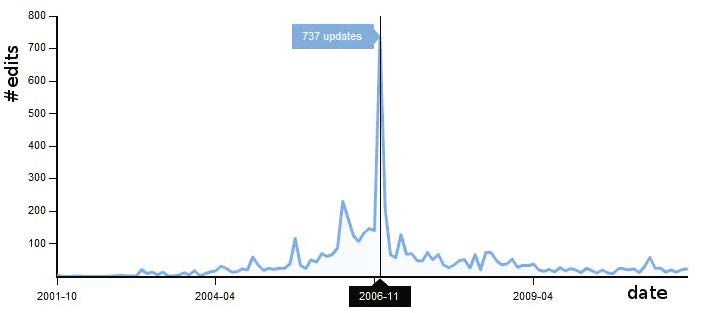
\includegraphics[width=.5\textwidth]{images/Extracting_EventRelated_Information_from_Article.jpg}
    \caption{Donald Rumsfeld’s Rücktritt führte zu einem Burst an Autoren, die einen Wikipedia-Edit vornahmen \cite{10.1007978-3-642-36973-5_22}.}
    \label{fig:donald_rumsfelds_resignation_burst}
\end{figure}